\documentclass[twoside]{book}

% Packages required by doxygen
\usepackage{fixltx2e}
\usepackage{calc}
\usepackage{doxygen}
\usepackage[export]{adjustbox} % also loads graphicx
\usepackage{graphicx}
\usepackage[utf8]{inputenc}
\usepackage{makeidx}
\usepackage{multicol}
\usepackage{multirow}
\PassOptionsToPackage{warn}{textcomp}
\usepackage{textcomp}
\usepackage[nointegrals]{wasysym}
\usepackage[table]{xcolor}

% Font selection
\usepackage[T1]{fontenc}
\usepackage[scaled=.90]{helvet}
\usepackage{courier}
\usepackage{amssymb}
\usepackage{sectsty}
\renewcommand{\familydefault}{\sfdefault}
\allsectionsfont{%
  \fontseries{bc}\selectfont%
  \color{darkgray}%
}
\renewcommand{\DoxyLabelFont}{%
  \fontseries{bc}\selectfont%
  \color{darkgray}%
}
\newcommand{\+}{\discretionary{\mbox{\scriptsize$\hookleftarrow$}}{}{}}

% Page & text layout
\usepackage{geometry}
\geometry{%
  a4paper,%
  top=2.5cm,%
  bottom=2.5cm,%
  left=2.5cm,%
  right=2.5cm%
}
\tolerance=750
\hfuzz=15pt
\hbadness=750
\setlength{\emergencystretch}{15pt}
\setlength{\parindent}{0cm}
\setlength{\parskip}{0.2cm}
\makeatletter
\renewcommand{\paragraph}{%
  \@startsection{paragraph}{4}{0ex}{-1.0ex}{1.0ex}{%
    \normalfont\normalsize\bfseries\SS@parafont%
  }%
}
\renewcommand{\subparagraph}{%
  \@startsection{subparagraph}{5}{0ex}{-1.0ex}{1.0ex}{%
    \normalfont\normalsize\bfseries\SS@subparafont%
  }%
}
\makeatother

% Headers & footers
\usepackage{fancyhdr}
\pagestyle{fancyplain}
\fancyhead[LE]{\fancyplain{}{\bfseries\thepage}}
\fancyhead[CE]{\fancyplain{}{}}
\fancyhead[RE]{\fancyplain{}{\bfseries\leftmark}}
\fancyhead[LO]{\fancyplain{}{\bfseries\rightmark}}
\fancyhead[CO]{\fancyplain{}{}}
\fancyhead[RO]{\fancyplain{}{\bfseries\thepage}}
\fancyfoot[LE]{\fancyplain{}{}}
\fancyfoot[CE]{\fancyplain{}{}}
\fancyfoot[RE]{\fancyplain{}{\bfseries\scriptsize Generated on Thu May 14 2015 01\+:17\+:13 for My Project by Doxygen }}
\fancyfoot[LO]{\fancyplain{}{\bfseries\scriptsize Generated on Thu May 14 2015 01\+:17\+:13 for My Project by Doxygen }}
\fancyfoot[CO]{\fancyplain{}{}}
\fancyfoot[RO]{\fancyplain{}{}}
\renewcommand{\footrulewidth}{0.4pt}
\renewcommand{\chaptermark}[1]{%
  \markboth{#1}{}%
}
\renewcommand{\sectionmark}[1]{%
  \markright{\thesection\ #1}%
}

% Indices & bibliography
\usepackage{natbib}
\usepackage[titles]{tocloft}
\setcounter{tocdepth}{3}
\setcounter{secnumdepth}{5}
\makeindex

% Hyperlinks (required, but should be loaded last)
\usepackage{ifpdf}
\ifpdf
  \usepackage[pdftex,pagebackref=true]{hyperref}
\else
  \usepackage[ps2pdf,pagebackref=true]{hyperref}
\fi
\hypersetup{%
  colorlinks=true,%
  linkcolor=blue,%
  citecolor=blue,%
  unicode%
}

% Custom commands
\newcommand{\clearemptydoublepage}{%
  \newpage{\pagestyle{empty}\cleardoublepage}%
}


%===== C O N T E N T S =====

\begin{document}

% Titlepage & ToC
\hypersetup{pageanchor=false,
             bookmarks=true,
             bookmarksnumbered=true,
             pdfencoding=unicode
            }
\pagenumbering{roman}
\begin{titlepage}
\vspace*{7cm}
\begin{center}%
{\Large My Project }\\
\vspace*{1cm}
{\large Generated by Doxygen 1.8.9.1}\\
\vspace*{0.5cm}
{\small Thu May 14 2015 01:17:13}\\
\end{center}
\end{titlepage}
\clearemptydoublepage
\tableofcontents
\clearemptydoublepage
\pagenumbering{arabic}
\hypersetup{pageanchor=true}

%--- Begin generated contents ---
\chapter{Class Index}
\section{Class List}
Here are the classes, structs, unions and interfaces with brief descriptions\+:\begin{DoxyCompactList}
\item\contentsline{section}{\hyperlink{classWarehouse}{Warehouse} }{\pageref{classWarehouse}}{}
\end{DoxyCompactList}

\chapter{File Index}
\section{File List}
Here is a list of all files with brief descriptions\+:\begin{DoxyCompactList}
\item\contentsline{section}{src/\hyperlink{main_8cpp}{main.\+cpp} }{\pageref{main_8cpp}}{}
\item\contentsline{section}{src/\hyperlink{warehouse_8cpp}{warehouse.\+cpp} }{\pageref{warehouse_8cpp}}{}
\item\contentsline{section}{src/\hyperlink{warehouse_8h}{warehouse.\+h} }{\pageref{warehouse_8h}}{}
\end{DoxyCompactList}

\chapter{Class Documentation}
\hypertarget{classWarehouse}{}\section{Warehouse Class Reference}
\label{classWarehouse}\index{Warehouse@{Warehouse}}


{\ttfamily \#include $<$warehouse.\+h$>$}

\subsection*{Public Member Functions}
\begin{DoxyCompactItemize}
\item 
\hyperlink{classWarehouse_af8d6c7e60cb3be65b35702b400e8fad7}{Warehouse} ()
\item 
void \hyperlink{classWarehouse_aea2ee7aeb732b03e14eaedd1a0cbfcd1}{put\+Goods} (int amount)
\item 
int \hyperlink{classWarehouse_ab3b8d5c4ed11911da0de65bec858173a}{take\+Goods} (int amount)
\item 
int \hyperlink{classWarehouse_a57befb61412bea93b4c5ed31636671fd}{get\+Stock} ()
\end{DoxyCompactItemize}


\subsection{Constructor \& Destructor Documentation}
\hypertarget{classWarehouse_af8d6c7e60cb3be65b35702b400e8fad7}{}\index{Warehouse@{Warehouse}!Warehouse@{Warehouse}}
\index{Warehouse@{Warehouse}!Warehouse@{Warehouse}}
\subsubsection[{Warehouse}]{\setlength{\rightskip}{0pt plus 5cm}Warehouse\+::\+Warehouse (
\begin{DoxyParamCaption}
{}
\end{DoxyParamCaption}
)}\label{classWarehouse_af8d6c7e60cb3be65b35702b400e8fad7}


\subsection{Member Function Documentation}
\hypertarget{classWarehouse_a57befb61412bea93b4c5ed31636671fd}{}\index{Warehouse@{Warehouse}!get\+Stock@{get\+Stock}}
\index{get\+Stock@{get\+Stock}!Warehouse@{Warehouse}}
\subsubsection[{get\+Stock}]{\setlength{\rightskip}{0pt plus 5cm}int Warehouse\+::get\+Stock (
\begin{DoxyParamCaption}
{}
\end{DoxyParamCaption}
)}\label{classWarehouse_a57befb61412bea93b4c5ed31636671fd}
\hypertarget{classWarehouse_aea2ee7aeb732b03e14eaedd1a0cbfcd1}{}\index{Warehouse@{Warehouse}!put\+Goods@{put\+Goods}}
\index{put\+Goods@{put\+Goods}!Warehouse@{Warehouse}}
\subsubsection[{put\+Goods}]{\setlength{\rightskip}{0pt plus 5cm}void Warehouse\+::put\+Goods (
\begin{DoxyParamCaption}
\item[{int}]{amount}
\end{DoxyParamCaption}
)}\label{classWarehouse_aea2ee7aeb732b03e14eaedd1a0cbfcd1}
\hypertarget{classWarehouse_ab3b8d5c4ed11911da0de65bec858173a}{}\index{Warehouse@{Warehouse}!take\+Goods@{take\+Goods}}
\index{take\+Goods@{take\+Goods}!Warehouse@{Warehouse}}
\subsubsection[{take\+Goods}]{\setlength{\rightskip}{0pt plus 5cm}int Warehouse\+::take\+Goods (
\begin{DoxyParamCaption}
\item[{int}]{amount}
\end{DoxyParamCaption}
)}\label{classWarehouse_ab3b8d5c4ed11911da0de65bec858173a}


The documentation for this class was generated from the following files\+:\begin{DoxyCompactItemize}
\item 
src/\hyperlink{warehouse_8h}{warehouse.\+h}\item 
src/\hyperlink{warehouse_8cpp}{warehouse.\+cpp}\end{DoxyCompactItemize}

\chapter{File Documentation}
\hypertarget{main_8cpp}{}\section{src/main.cpp File Reference}
\label{main_8cpp}\index{src/main.\+cpp@{src/main.\+cpp}}
{\ttfamily \#include $<$stdio.\+h$>$}\\*
Include dependency graph for main.\+cpp\+:
\nopagebreak
\begin{figure}[H]
\begin{center}
\leavevmode
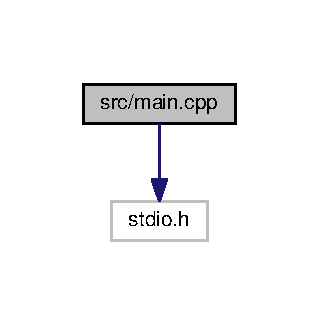
\includegraphics[width=153pt]{main_8cpp__incl}
\end{center}
\end{figure}
\subsection*{Functions}
\begin{DoxyCompactItemize}
\item 
int \hyperlink{main_8cpp_ae66f6b31b5ad750f1fe042a706a4e3d4}{main} ()
\end{DoxyCompactItemize}


\subsection{Function Documentation}
\hypertarget{main_8cpp_ae66f6b31b5ad750f1fe042a706a4e3d4}{}\index{main.\+cpp@{main.\+cpp}!main@{main}}
\index{main@{main}!main.\+cpp@{main.\+cpp}}
\subsubsection[{main}]{\setlength{\rightskip}{0pt plus 5cm}int main (
\begin{DoxyParamCaption}
{}
\end{DoxyParamCaption}
)}\label{main_8cpp_ae66f6b31b5ad750f1fe042a706a4e3d4}

\hypertarget{warehouse_8cpp}{}\section{src/warehouse.cpp File Reference}
\label{warehouse_8cpp}\index{src/warehouse.\+cpp@{src/warehouse.\+cpp}}
{\ttfamily \#include \char`\"{}warehouse.\+h\char`\"{}}\\*
Include dependency graph for warehouse.\+cpp\+:
\nopagebreak
\begin{figure}[H]
\begin{center}
\leavevmode
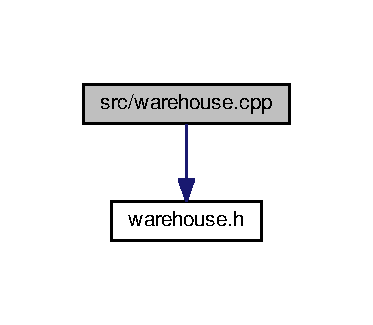
\includegraphics[width=179pt]{warehouse_8cpp__incl}
\end{center}
\end{figure}

\hypertarget{warehouse_8h}{}\section{src/warehouse.h File Reference}
\label{warehouse_8h}\index{src/warehouse.\+h@{src/warehouse.\+h}}
This graph shows which files directly or indirectly include this file\+:
\nopagebreak
\begin{figure}[H]
\begin{center}
\leavevmode
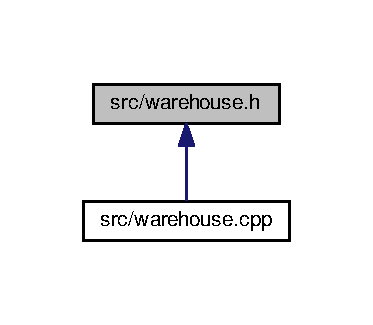
\includegraphics[width=179pt]{warehouse_8h__dep__incl}
\end{center}
\end{figure}
\subsection*{Classes}
\begin{DoxyCompactItemize}
\item 
class \hyperlink{classWarehouse}{Warehouse}
\end{DoxyCompactItemize}

%--- End generated contents ---

% Index
\backmatter
\newpage
\phantomsection
\clearemptydoublepage
\addcontentsline{toc}{chapter}{Index}
\printindex

\end{document}
